%%
%% This is file `sample-sigconf-authordraft.tex',
%% generated with the docstrip utility.
%%
%% The original source files were:
%%
%% samples.dtx  (with options: `all,proceedings,bibtex,authordraft')
%% 
%% IMPORTANT NOTICE:
%% 
%% For the copyright see the source file.
%% 
%% Any modified versions of this file must be renamed
%% with new filenames distinct from sample-sigconf-authordraft.tex.
%% 
%% For distribution of the original source see the terms
%% for copying and modification in the file samples.dtx.
%% 
%% This generated file may be distributed as long as the
%% original source files, as listed above, are part of the
%% same distribution. (The sources need not necessarily be
%% in the same archive or directory.)
%%
%%
%% Commands for TeXCount
%TC:macro \cite [option:text,text]
%TC:macro \citep [option:text,text]
%TC:macro \citet [option:text,text]
%TC:envir table 0 1
%TC:envir table* 0 1
%TC:envir tabular [ignore] word
%TC:envir displaymath 0 word
%TC:envir math 0 word
%TC:envir comment 0 0
%%
%% The first command in your LaTeX source must be the \documentclass
%% command.
%%
%% For submission and review of your manuscript please change the
%% command to \documentclass[manuscript, screen, review]{acmart}.
%%
%% When submitting camera ready or to TAPS, please change the command
%% to \documentclass[sigconf]{acmart} or whichever template is required
%% for your publication.
%%
%%

\documentclass[sigconf,authordraft]{acmart}
%%
%% \BibTeX command to typeset BibTeX logo in the docs
\AtBeginDocument{%
  \providecommand\BibTeX{{%
    Bib\TeX}}}

%% Rights management information.  This information is sent to you
%% when you complete the rights form.  These commands have SAMPLE
%% values in them; it is your responsibility as an author to replace
%% the commands and values with those provided to you when you
%% complete the rights form.
\setcopyright{acmlicensed}
\copyrightyear{2026}
\acmYear{2026}
\acmDOI{}
%% These commands are for a PROCEEDINGS abstract or paper.
\acmConference[WADS '26]{Workshop on Algorithms and Data Structures}{August 05--07, 2026}{Ljubljana, Slovenia}
\acmISBN{978-x-xxxx-xxxx-x/26/08}

\renewcommand{\abstractname}{Povzetek}
\renewcommand{\keywordsname}{Ključne besede}
\renewcommand{\refname}{Literatura}
\renewcommand{\bibname}{Literatura}

%%
%% Submission ID.
%% Use this when submitting an article to a sponsored event. You'll
%% receive a unique submission ID from the organizers
%% of the event, and this ID should be used as the parameter to this command.
%%\acmSubmissionID{123-A56-BU3}

%%
%% For managing citations, it is recommended to use bibliography
%% files in BibTeX format.
%%
%% You can then either use BibTeX with the ACM-Reference-Format style,
%% or BibLaTeX with the acmnumeric or acmauthoryear sytles, that include
%% support for advanced citation of software artefact from the
%% biblatex-software package, also separately available on CTAN.
%%
%% Look at the sample-*-biblatex.tex files for templates showcasing
%% the biblatex styles.
%%

%%
%% The majority of ACM publications use numbered citations and
%% references.  The command \citestyle{authoryear} switches to the
%% "author year" style.
%%
%% If you are preparing content for an event
%% sponsored by ACM SIGGRAPH, you must use the "author year" style of
%% citations and references.
%% Uncommenting
%% the next command will enable that style.
%%\citestyle{acmauthoryear}
\usepackage{tikz}
\usepackage[slovene]{babel}
\usetikzlibrary{graphs, graphs.standard, positioning}

%%
%% end of the preamble, start of the body of the document source.
\begin{document}

%%
%% The "title" command has an optional parameter,
%% allowing the author to define a "short title" to be used in page headers.
\title{Preverjanje konveksnosti ali izometričnosti podgrafa}

%%
%% The "author" command and its associated commands are used to define
%% the authors and their affiliations.
%% Of note is the shared affiliation of the first two authors, and the
%% "authornote" and "authornotemark" commands
%% used to denote shared contribution to the research.
\author{Bojan Dogandžić}
\email{bd21530@student.uni-lj.si}
\affiliation{%
  \institution{Univerza v Ljubljani, Fakulteta za računalništvo in informatiko}
  \city{Ljubljana}
  \country{Slovenija}
}

\author{Marko Horvat}
\email{mh3269@student.uni-lj.si}
\affiliation{%
  \institution{Univerza v Ljubljani, Fakulteta za računalništvo in informatiko}
  \city{Ljubljana}
  \country{Slovenija}
}

\author{Nejc Narobe}
\email{nn00483@student.uni-lj.si}
\affiliation{%
  \institution{Univerza v Ljubljani, Fakulteta za računalništvo in informatiko}
  \city{Ljubljana}
  \country{Slovenija}
}

\author{Marko Zupančič Muc}
\email{mzxxxx@student.uni-lj.si}
\affiliation{%
  \institution{Univerza v Ljubljani, Fakulteta za računalništvo in informatiko}
  \city{Ljubljana}
  \country{Slovenija}
}

%%
%% By default, the full list of authors will be used in the page
%% headers. Often, this list is too long, and will overlap
%% other information printed in the page headers. This command allows
%% the author to define a more concise list
%% of authors' names for this purpose.
\renewcommand{\shortauthors}{Dogandžić, et al.}

%%
%% The abstract is a short summary of the work to be presented in the
%% article.
\begin{abstract}
  A clear and well-documented \LaTeX\ document is presented as an
  article formatted for publication by ACM in a conference proceedings
  or journal publication. Based on the ``acmart'' document class, this
  article presents and explains many of the common variations, as well
  as many of the formatting elements an author may use in the
  preparation of the documentation of their work.
\end{abstract}

%%
%% The code below is generated by the tool at http://dl.acm.org/ccs.cfm.
%% Please copy and paste the code instead of the example below.
%%
\begin{CCSXML}
<ccs2012>
   <concept>
       <concept_id>10003752.10003809.10003635</concept_id>
       <concept_desc>Theory of computation~Graph algorithms analysis</concept_desc>
       <concept_significance>500</concept_significance>
       </concept>
   <concept>
       <concept_id>10002950.10003624.10003633.10003637</concept_id>
       <concept_desc>Mathematics of computing~Graph theory</concept_desc>
       <concept_significance>500</concept_significance>
       </concept>
   <concept>
       <concept_id>10003752.10003809.10003716</concept_id>
       <concept_desc>Theory of computation~Mathematical optimization</concept_desc>
       <concept_significance>300</concept_significance>
       </concept>
 </ccs2012>
\end{CCSXML}

\ccsdesc[500]{Theory of computation~Graph algorithms analysis}
\ccsdesc[500]{Mathematics of computing~Graph theory}
\ccsdesc[300]{Theory of computation~Mathematical optimization}

%%
%% Keywords. The author(s) should pick words that accurately describe
%% the work being presented. Separate the keywords with commas.
\keywords{konveksnost, izometričnost, podgrafi, algoritmi}
%% A "teaser" image appears between the author and affiliation
%% information and the body of the document, and typically spans the
%% page.
\begin{teaserfigure}
  \centering
  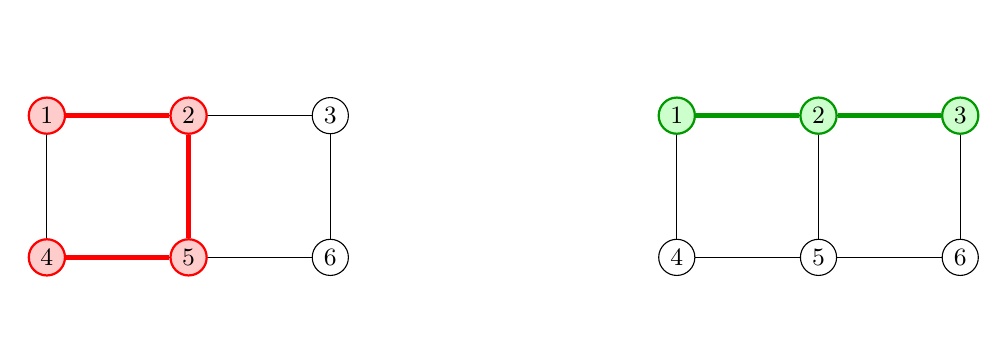
\begin{tikzpicture}[node distance=1.8cm, main/.style = {draw, circle, inner sep=2pt, font=\small}]
    \begin{scope}[xshift=-4cm]
      \node[font=\bfseries] at (1.2, 1) {};
      \node[main] (G1) {1}; \node[main] (G2) [right of=G1] {2}; \node[main] (G3) [right of=G2] {3};
      \node[main] (G4) [below of=G1] {4}; \node[main] (G5) [right of=G4] {5}; \node[main] (G6) [right of=G5] {6};
      \draw (G1)--(G2)--(G3); \draw (G4)--(G5)--(G6); \draw (G1)--(G4); \draw (G2)--(G5); \draw (G3)--(G6);
      \begin{scope}[every node/.style={main, fill=red!20, draw=red, thick}]
        \node (H1) at (0,0) {1}; \node (H2) at (1.8,0) {2}; \node (H5) at (1.8,-1.8) {5}; \node (H4) at (0,-1.8) {4};
      \end{scope}
      \draw[red, ultra thick] (H1)--(H2)--(H5)--(H4)--cycle;
      \node at (1.2, -2.5) {};
    \end{scope}
    \begin{scope}[xshift=4cm]
      \node[font=\bfseries] at (1.2, 1) {};
      \node[main] (GK1) {1}; \node[main] (GK2) [right of=GK1] {2}; \node[main] (GK3) [right of=GK2] {3};
      \node[main] (GK4) [below of=GK1] {4}; \node[main] (GK5) [right of=GK4] {5}; \node[main] (GK6) [right of=GK5] {6};
      \draw (GK1)--(GK2)--(GK3); \draw (GK4)--(GK5)--(GK6); \draw (GK1)--(GK4); \draw (GK2)--(GK5); \draw (GK3)--(GK6);
      \begin{scope}[every node/.style={main, fill=green!20, draw=green!60!black, thick}]
        \node (K1) at (0,0) {1}; \node (K2) at (1.8,0) {2}; \node (K3) at (3.6,0) {3};
      \end{scope}
      \draw[green!60!black, ultra thick] (K1)--(K2)--(K3);
      \node at (1.8, -2.5) {};
    \end{scope}
  \end{tikzpicture}
  \caption{Primer izometričnega in konveksnega podgrafa.}
  \label{fig:teaser}
\end{teaserfigure}

%%
%% This command processes the author and affiliation and title
%% information and builds the first part of the formatted document.
\maketitle

\section{Uvod}
Teorija grafov predstavlja temelj za razumevanje kompleksnih struktur v modernem računalništvu, od topologij računalniških omrežij do analize socialnih interakcij. Razumevanje grafov in izvajanje algoritmov nad njimi omogoča učinkovito ter avtomatizirano analizo tudi na številnih drugih področjih izven čiste računalniške znanosti, kot so biologija, kemija in logistika.
\\
Eden ključnih izzivov pri delu z obsežnimi grafovnimi strukturami je prepoznavanje lastnosti posameznih podgrafov. V tem kontekstu sta izjemno pomembni lastnosti izometričnost in konveksnost. Izometrični podgrafi, ki jih je med prvimi podrobneje raziskoval Djoković \cite{djokovic1973}, ohranjajo razdalje med vozlišči, kar pomeni, da je najkrajša pot med poljubnima vozliščema v podgrafu enako dolga kot v celotnem grafu. Konveksni podgrafi pa predstavljajo še strožji pogoj, saj zahtevajo, da so prav vse najkrajše poti med vozlišči podgrafa v celoti vsebovane znotraj njega.
\\
Preverjanje omenjenih lastnosti na prvi pogled deluje preprosto, vendar se pri naivnem pristopu hitro soočimo s problemom računske zahtevnosti. Naivna metoda bi namreč zahtevala izračun najkrajših poti med vsemi pari vozlišč v podgrafu (ang. \textit{All-Pairs Shortest Paths}) in njihovo primerjavo z razdaljami v izvornem grafu. Takšen pristop ima časovno zahtevnost vsaj $O(n^3)$ ali $O(n^2 \log n + nm)$, kar je pri grafih z več tisoč vozlišči praktično neuporabno. Iskanje učinkovitejših algoritmov, ki bi izkoristili specifične strukturne lastnosti grafov, je zato ključno za razvoj odzivnih sistemov.
\\
Razumevanje teh struktur je odločilno za optimizacijo usmerjanja v mrežah (ang. \textit{routing}) in za razvoj naprednih algoritmov v računalniški geometriji. V tem eseju se podrobneje osredotočamo na članek \cite{main_paper}, ki analizira algoritme za učinkovito preverjanje teh dveh lastnosti. Naš namen je ne le povzeti predstavljene algoritme, temveč tudi kritično ovrednotiti njihovo uporabnost pri specifičnih topologijah. V nadaljevanju bomo najprej definirali ključne pojme, nato analizirali obstoječe rešitve, v poglavju \ref{sec:premislek} pa predstavili lastne predloge za nadgradnjo in eksperimentalno ovrednotenje teh pristopov.
\section{Osnove in definicije}
\subsection{Izometrični podgrafi}

\subsection{Konveksni podgrafi}

\section{Pregled področja}
\subsection{Zgodovinski razvoj in sorodni problemi}
\subsection{Pregled obstoječih algoritmov}
\section{Premislek in teoretična nadgradnja}

\section{Eksperimentalno ovrednotenje}

\section{Zaključek}

\bibliographystyle{ACM-Reference-Format}
\bibliography{sample-base}


%%
%% If your work has an appendix, this is the place to put it.
\appendix



\end{document}
\endinput
%%
%% End of file `sample-sigconf-authordraft.tex'.
